\documentclass{standalone}
\usepackage{tikz}
\usepackage{pgfplots}
\pgfplotsset{compat=1.16}

\begin{document}
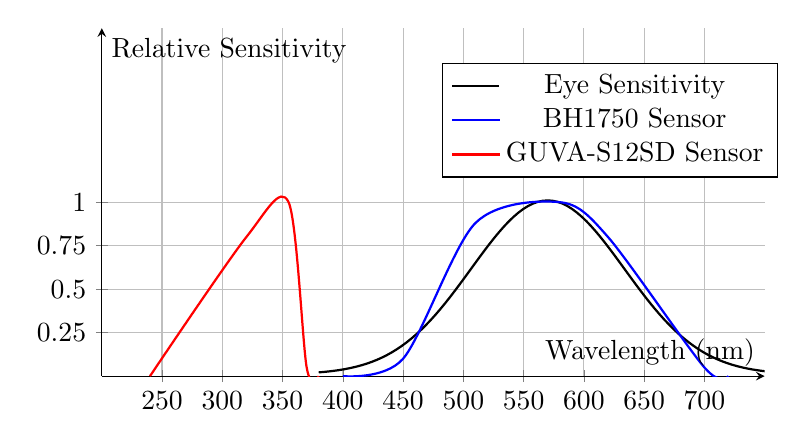
\begin{tikzpicture}
\begin{axis}[
    xlabel={Wavelength (nm)},
    ylabel={Relative Sensitivity},
    ylabel style={rotate=-90},
    ymin=0,
    ymax=2,
    xmin=200,
    xmax=750,
    xtick={250, 300,350, 400, 450, 500, 550, 600, 650, 700},
    xticklabels={250, 300,350, 400, 450, 500, 550, 600, 650, 700},
    ytick={0, 0.25, 0.5, 0.75, 1},
    yticklabels={0, 0.25, 0.5, 0.75, 1},
    grid=both,
    axis lines=middle,
    width=10cm,
    height=6cm,
    legend style={at={(1.02,0.9)}, anchor=north east},
]
\addplot[black, thick, domain=380:780, samples=100] {0.01+exp(-((x-570)/90)^2)};
\addplot[blue, thick, smooth] coordinates {
    (400, 0)
    (450, 0.1)
    (510, 0.88)
    (580, 1)
    (620, 0.8)
    (700, 0.05)
    (720, 0)
};
\addplot[red, thick, smooth] coordinates {
    (240, 0)
    (320, 0.8)
    (355, 1)
    (370, 0.05)
    (380, 0)
};

\legend{Eye Sensitivity, BH1750 Sensor, GUVA-S12SD Sensor}
\end{axis}
\end{tikzpicture}
\end{document}

